%% ============================================================================
%%  Machine Learning: Science and Technology (IOP Publishing) — submission source
%%  Paper 1, version 2 (revised).
%%  Class: iopjournal.cls  (IOP Publishing 2025 official template; obtain from
%%         https://publishingsupport.iopscience.iop.org/ -> "LaTeX template".
%%         Place iopjournal.cls in this folder, or install into your TeX tree.)
%%  Engine: pdflatex  (run twice for cross-references)
%%  Figures: figure1.png (anatomy), figure2.png (null decomposition),
%%           figure3.png (cross-dataset summary), figure4.png (family ceiling)
%%           — all in same folder
%% ============================================================================
\documentclass{iopjournal}

% --- packages beyond those the class already loads (graphicx, xcolor, hyperref, fancyhdr) ---
\usepackage[T1]{fontenc}   % ogonek in Szcz\k{e}\'sniak (ref. wrona2024) needs T1, not OT1
\usepackage{amsmath}
\usepackage{amssymb}
\usepackage{booktabs}
\usepackage{siunitx}
\usepackage{url}

\sisetup{detect-weight=true, detect-family=true, table-number-alignment=center}

\newcommand{\Tc}{T_{\mathrm c}}
\newcommand{\Rsq}{R^{2}}
\newcommand{\etal}{\textit{et al}}
\newcommand{\ICC}{\mathrm{ICC}}
\newcommand{\Neff}{N_{\mathrm{eff}}}

\begin{document}

\articletype{Paper}

\title{Random splits inflate the accuracy of composition-based superconductor
$\Tc$ models: a leakage-aware evaluation replicated across two datasets}

\author{Gabriel Jaime Cardona Osorio\orcid{0009-0003-3743-8559}}

\affil{Faculty of Engineering, Instituci\'on Universitaria Pascual Bravo, Medell\'in, Colombia}

\email{gabriel.cardona@pascualbravo.edu.co}

\keywords{superconductivity, critical temperature, machine learning, materials informatics,
data leakage, cross-validation, cluster sampling, design effect}

\begin{abstract}
Composition-based machine-learning models routinely report $\Rsq \approx 0.93$ and
MAE $\approx \SI{5}{\kelvin}$ for superconducting critical temperature, but these figures are
obtained by splitting datasets at the level of the individual compound. Superconductor datasets
are not samples of independent compounds: they are assembled from doping series, so a random
split places near-identical stoichiometric variants of the same chemistry on both sides of the
partition. We quantify what that costs. Holding out whole chemical families---materials sharing
a constituent-element set---inflates MAE by \SIrange{52}{61}{\percent} and lowers $\Rsq$ by
\numrange{0.071}{0.081} across two independently curated datasets
(\num{21263} and \num{12440} compounds) and two featurizations, with the effect measured over
five independent partitions. We then ask what the inflated number was measuring. Treating family
identity as a clustering variable, the intraclass correlation of $\Tc$ within a family is
\num{0.85} in both datasets, giving a cluster design effect of \numrange{3.6}{5.5} and an
effective sample size (\num{3847} and \num{3470}) within \SI{14}{\percent} of the number of
chemical families rather than the number of compounds. In-sample, family identity alone---no
chemistry, no descriptors---accounts for \SI{87.7}{\percent} and \SI{88.4}{\percent} of the
variance in $\Tc$, which is the share of the target that a categorical label already explains.
Screening utility,
however, survives: under family-held-out validation the top-100 precision remains
\SI{87.0}{\percent} and \SI{85.2}{\percent} against a \SI{10}{\percent} base rate, while a
family-mean lookup collapses to chance (\SI{11.6}{\percent} and \SI{9.6}{\percent}). The
correction is one extra cross-validation run, and we release deterministic family splits and
code so it can be adopted as a reporting standard.
\end{abstract}

\section{Introduction}

Predicting the superconducting critical temperature $\Tc$ from chemical composition alone is one
of the most-benchmarked regression tasks in materials informatics. The headline numbers are
consistently strong: gradient-boosted trees and random forests on the Hamidieh
featurization~\cite{hamidieh2018} or on Magpie descriptors~\cite{ward2016} report
$\Rsq \gtrsim 0.92$ and MAE below \SI{6}{\kelvin}, and deep architectures push the same metrics
further~\cite{konno2021,zeng2019,stanev2018}. Those numbers are quoted when arguing that
machine learning is ready to guide the search for new superconductors, and models of this class
have been used to propose candidates from text-mined phase diagrams~\cite{court2020}, from
Eliashberg-theory descriptors~\cite{xie2022}, and to screen hydride
families~\cite{sanna2024,wrona2024}.

They are also obtained in a way that does not resemble the search. The datasets used are derived
from SuperCon and are assembled from \emph{doping series}: families of materials that share a
constituent-element set and differ only in stoichiometry. A YBa$_2$Cu$_3$O$_{7-\delta}$ series
contributes dozens of entries whose compositions differ in the third decimal place of the oxygen
content and whose $\Tc$ values differ by a few kelvin. When such a dataset is split at random,
near-identical twins of every test compound sit in the training set. The resulting metric measures
interpolation within a series the model has already seen. A discovery campaign asks the opposite
question: what is $\Tc$ for a chemistry that has never been synthesised?

The general form of this problem is well known. Meredig \etal~\cite{meredig2018} introduced
leave-one-cluster-out cross-validation for materials discovery and showed that extrapolative
performance is systematically worse than the interpolative figure. Kapoor and
Narayanan~\cite{kapoor2023} document leakage from non-independent samples as a recurring failure
mode across machine-learning-based science. The Matbench efforts~\cite{dunn2020,riebesell2024}
make the related point that strong regression metrics need not translate into discovery utility.
What has been missing for superconductors specifically is a quantitative answer to three
questions: which grouping is the right one for this domain, how large the gap is, and whether the
gap is a property of one dataset or of the task.

This paper answers all three, and then asks a fourth question that the leakage framing does not
by itself address. Sections~\ref{sec:results-gap} and~\ref{sec:results-robust} establish the gap
and its stability. Section~\ref{sec:results-ceiling} asks what the inflated number was actually
measuring, and finds that family identity alone---a variable containing no chemical information
beyond a label---accounts for almost all of it. Section~\ref{sec:results-screening} shows that
the practical screening application nonetheless survives, so the correct conclusion is a
recalibration rather than a dismissal.

Our contributions are:
\begin{enumerate}
\item A domain-appropriate grouping variable: the constituent-element set, which corresponds
      one-to-one with the doping series that generate the redundancy, and which can be verified
      by inspection rather than assumed from an unsupervised clustering.
\item A measurement of the resulting gap, replicated across two independently curated datasets
      with two different featurizations and evaluated over five independent partitions.
\item A reframing of the gap in cluster-sampling terms: the intraclass correlation, design effect
      and effective sample size of each dataset, which quantify the inflation in a
      model-independent and protocol-independent way.
\item A ladder of nulls---family-mean lookup, element-presence indicators, full descriptors---that
      separates memorisation from learned chemistry, and shows that screening skill is genuine
      while most of the variance the conventional $\Rsq$ rewards is already available from a
      family label.
\item Deterministic, released family splits and the code to reproduce every number, so that the
      corrected protocol costs one command.
\end{enumerate}

\section{Data and methods}

\subsection{Datasets}
\label{sec:data}

\textbf{Dataset~A} is the UCI Superconductivity Data Set~\cite{hamidieh2018}: \num{21263}
compounds with \num{81} statistical features derived from elemental properties (mean, weighted
mean, geometric mean, entropy, range and standard deviation of atomic mass, ionisation energy,
atomic radius, density, electron affinity, fusion heat, thermal conductivity and valence),
accompanied by a per-element composition table giving the chemical formula of each entry.

\textbf{Dataset~B} is the SuperCon-derived list curated by Stanev \etal~\cite{stanev2018}. We
retain entries with $\Tc > 0$ and a formula parseable by \texttt{pymatgen}, yielding \num{12440}
compounds, and featurize them with the \num{132} Magpie descriptors~\cite{ward2016} as
implemented in \texttt{matminer}~\cite{ward2018}.

The two datasets share a common ancestry in SuperCon but differ in curation, in size, and
entirely in featurization. Agreement between them is therefore evidence about the task rather
than about a particular data-processing choice.

\subsection{Chemical families}
\label{sec:families}

We define a \emph{chemical family} as the set of constituent elements of a compound, irrespective
of stoichiometry: Ba$_{0.2}$La$_{1.8}$Cu$_{1}$O$_{4}$ and Ba$_{0.1}$La$_{1.9}$Cu$_{1}$O$_{4}$
both belong to the family $\{$Ba, La, Cu, O$\}$. This is the grouping that corresponds to the
doping series responsible for the redundancy, and unlike an unsupervised clustering it is
inspectable: a reader can verify family membership from the formula.

The resulting concentration is severe (figure~\ref{fig:anatomy}(a)). Dataset~A contains
\num{3365} families for \num{21263} compounds, with \SI{79.5}{\percent} of all materials in
families of five or more members; the three largest families hold \num{720}, \num{358} and
\num{323} compounds. Dataset~B contains \num{3063} families for \num{12440} compounds, with
\SI{66.7}{\percent} in families of five or more and a largest family of \num{131}. Both datasets
also carry a long tail of singletons (\num{1169} and \num{1322} respectively).

Family labels are assigned with \texttt{pandas.factorize} applied \emph{after} all row filtering.
This ordering matters: applying it before a $\Tc>0$ mask leaves gaps in the label sequence, and
because \texttt{GroupKFold} breaks ties by label order when assigning groups to folds, gapped and
contiguous labellings produce different partitions of the same families. We return to this point
in section~\ref{sec:repro}.

\subsection{Cross-validation protocols}
\label{sec:protocols}

We compare two protocols, identical in every respect except how the partition is formed:

\begin{itemize}
\item \textbf{Random}: \texttt{KFold(5, shuffle=True)}. Compounds are assigned to folds
      independently, so members of the same family routinely appear on both sides.
\item \textbf{Chemical-family}: \texttt{GroupKFold(5)} with the family label as the grouping
      variable. Every family appears in exactly one fold, so no test compound shares a chemistry
      with any training compound.
\end{itemize}

For the robustness analysis of section~\ref{sec:results-robust} both protocols are repeated over
five seeds. We use \texttt{GroupKFold(n\_splits=5, shuffle=True, random\_state=s)}, available
since scikit-learn~1.6, so that the grouped partition genuinely varies with the seed; without
\texttt{shuffle} the grouped splitter is deterministic and repeated runs differ only in model
initialisation.

\subsection{Models}

We use the two tree ensembles that dominate reported results on this task, with
hyperparameters fixed per dataset from prior grid searches and held constant across protocols.
Dataset~A: XGBoost~\cite{chen2016} with \num{250} estimators, maximum depth \num{8}, learning
rate \num{0.07}, subsample \num{0.9}, column subsample \num{0.7}, \texttt{gamma} \num{0},
\texttt{reg\_alpha} \num{0.01}; random forest with \num{150} trees, maximum depth \num{25} and
\texttt{sqrt} feature subsampling. Dataset~B: XGBoost with \num{300} estimators, maximum depth
\num{10}, learning rate \num{0.05}, subsample and column subsample \num{0.8}, \texttt{hist} tree
method; random forest with \num{150} trees and maximum depth \num{30}, without feature
subsampling. Both forests use \texttt{min\_samples\_leaf} \num{3} and
\texttt{min\_samples\_split} \num{5}. The two configurations differ because each was tuned
against its own featurization; they are held fixed across protocols, which is what the
random-versus-grouped comparison requires. Regression metrics (MAE, RMSE, $\Rsq$) are computed
on pooled out-of-fold predictions.

\subsection{Nulls and the family-identity ceiling}
\label{sec:nulls}

To separate memorisation from learned chemistry we evaluate a ladder of three predictors under
both protocols, on identical folds:

\begin{enumerate}
\item \textbf{Family-mean null.} No features at all: predict the mean $\Tc$ of the compound's
      family as computed on the training fold, falling back to the global training mean for
      unseen families. This is a pure lookup table.
\item \textbf{Element-presence null.} The same XGBoost, trained on binary indicators of element
      presence only (\num{86} indicators for Dataset~A, \num{83} for Dataset~B): does the
      compound contain Cu, does it contain O, and so on. All statistical and Magpie descriptors,
      and all stoichiometric information, are discarded.
\item \textbf{Full model.} The published featurization.
\end{enumerate}

Separately, we quantify how much of the variance in $\Tc$ is attributable to family identity
alone, treating the dataset as a clustered sample. With $N$ compounds in $k$ families of sizes
$n_i$, a one-way random-effects ANOVA gives the intraclass correlation
\begin{equation}
\ICC = \frac{\mathrm{MS_B} - \mathrm{MS_W}}{\mathrm{MS_B} + (m_0 - 1)\,\mathrm{MS_W}},
\qquad
m_0 = \frac{N - \sum_i n_i^2 / N}{k - 1},
\label{eq:icc}
\end{equation}
where $m_0$ is Searle's cluster size for unequal clusters. The corresponding design effect and
effective sample size are
\begin{equation}
\mathrm{deff} = 1 + (m - 1)\,\ICC,
\qquad
\Neff = N / \mathrm{deff},
\label{eq:deff}
\end{equation}
which we report for both $m = \bar m = N/k$ and $m = m_0$. We also report the oracle bound
$\eta^2 = 1 - \mathrm{SS_{within}}/\mathrm{SS_{total}}$ obtained from family means computed on
the full dataset. We emphasise that $\eta^2$ is \emph{not} a cross-validated $\Rsq$: it is
computed with knowledge of every family's mean, including families that a cross-validated model
would never see. It measures how much of the target a categorical label explains in-sample, and it
is not commensurable with a cross-validated score in either direction: the grouped-CV figures of
table~\ref{tab:main} fall below it while the random-split figures exceed it. We therefore never
take differences or ratios between $\eta^2$ and any $\Rsq$, and plot it with distinct hatching
throughout.

\subsection{Screening metric}
\label{sec:screening}

Discovery campaigns rank candidates rather than predicting each $\Tc$ exactly, so we also report
top-100 precision: the fraction of the \num{100} highest-predicted test compounds whose true
$\Tc$ exceeds a high-$\Tc$ threshold. We define that threshold as the 90th percentile of $\Tc$
\emph{within the training fold}, so the base rate is \SI{10}{\percent} by construction and no
information from the test fold enters the evaluation criterion. Using the whole-dataset
percentile instead changes the Dataset~B grouped figure by \num{0.4} points, but it would let
test compounds influence the threshold that judges them---the same class of leakage this paper
is about. Precision is reported as the mean over folds with the between-fold standard deviation;
features are not standardised.

\subsection{Nearest-neighbour diagnostic}

To confirm that the two protocols differ in the way the family construction predicts, we measure
the Euclidean distance from each test compound to its nearest training compound in standardised
feature space, under a random $80/20$ hold-out and under a grouped hold-out of the same size.

\section{Results}

\subsection{Reproducing the reported performance}
\label{sec:results-repro}

Under the conventional protocol our models match the published range. A single random $80/20$
split gives MAE $=\SI{5.14}{\kelvin}$ and $\Rsq = 0.932$ on Dataset~A, and
MAE $=\SI{3.76}{\kelvin}$ with $\Rsq = 0.934$ on Dataset~B. These are the figures a reader of
the literature would expect, and they establish that what follows is not an artefact of a weak
baseline.

\begin{figure}[t]
\centering
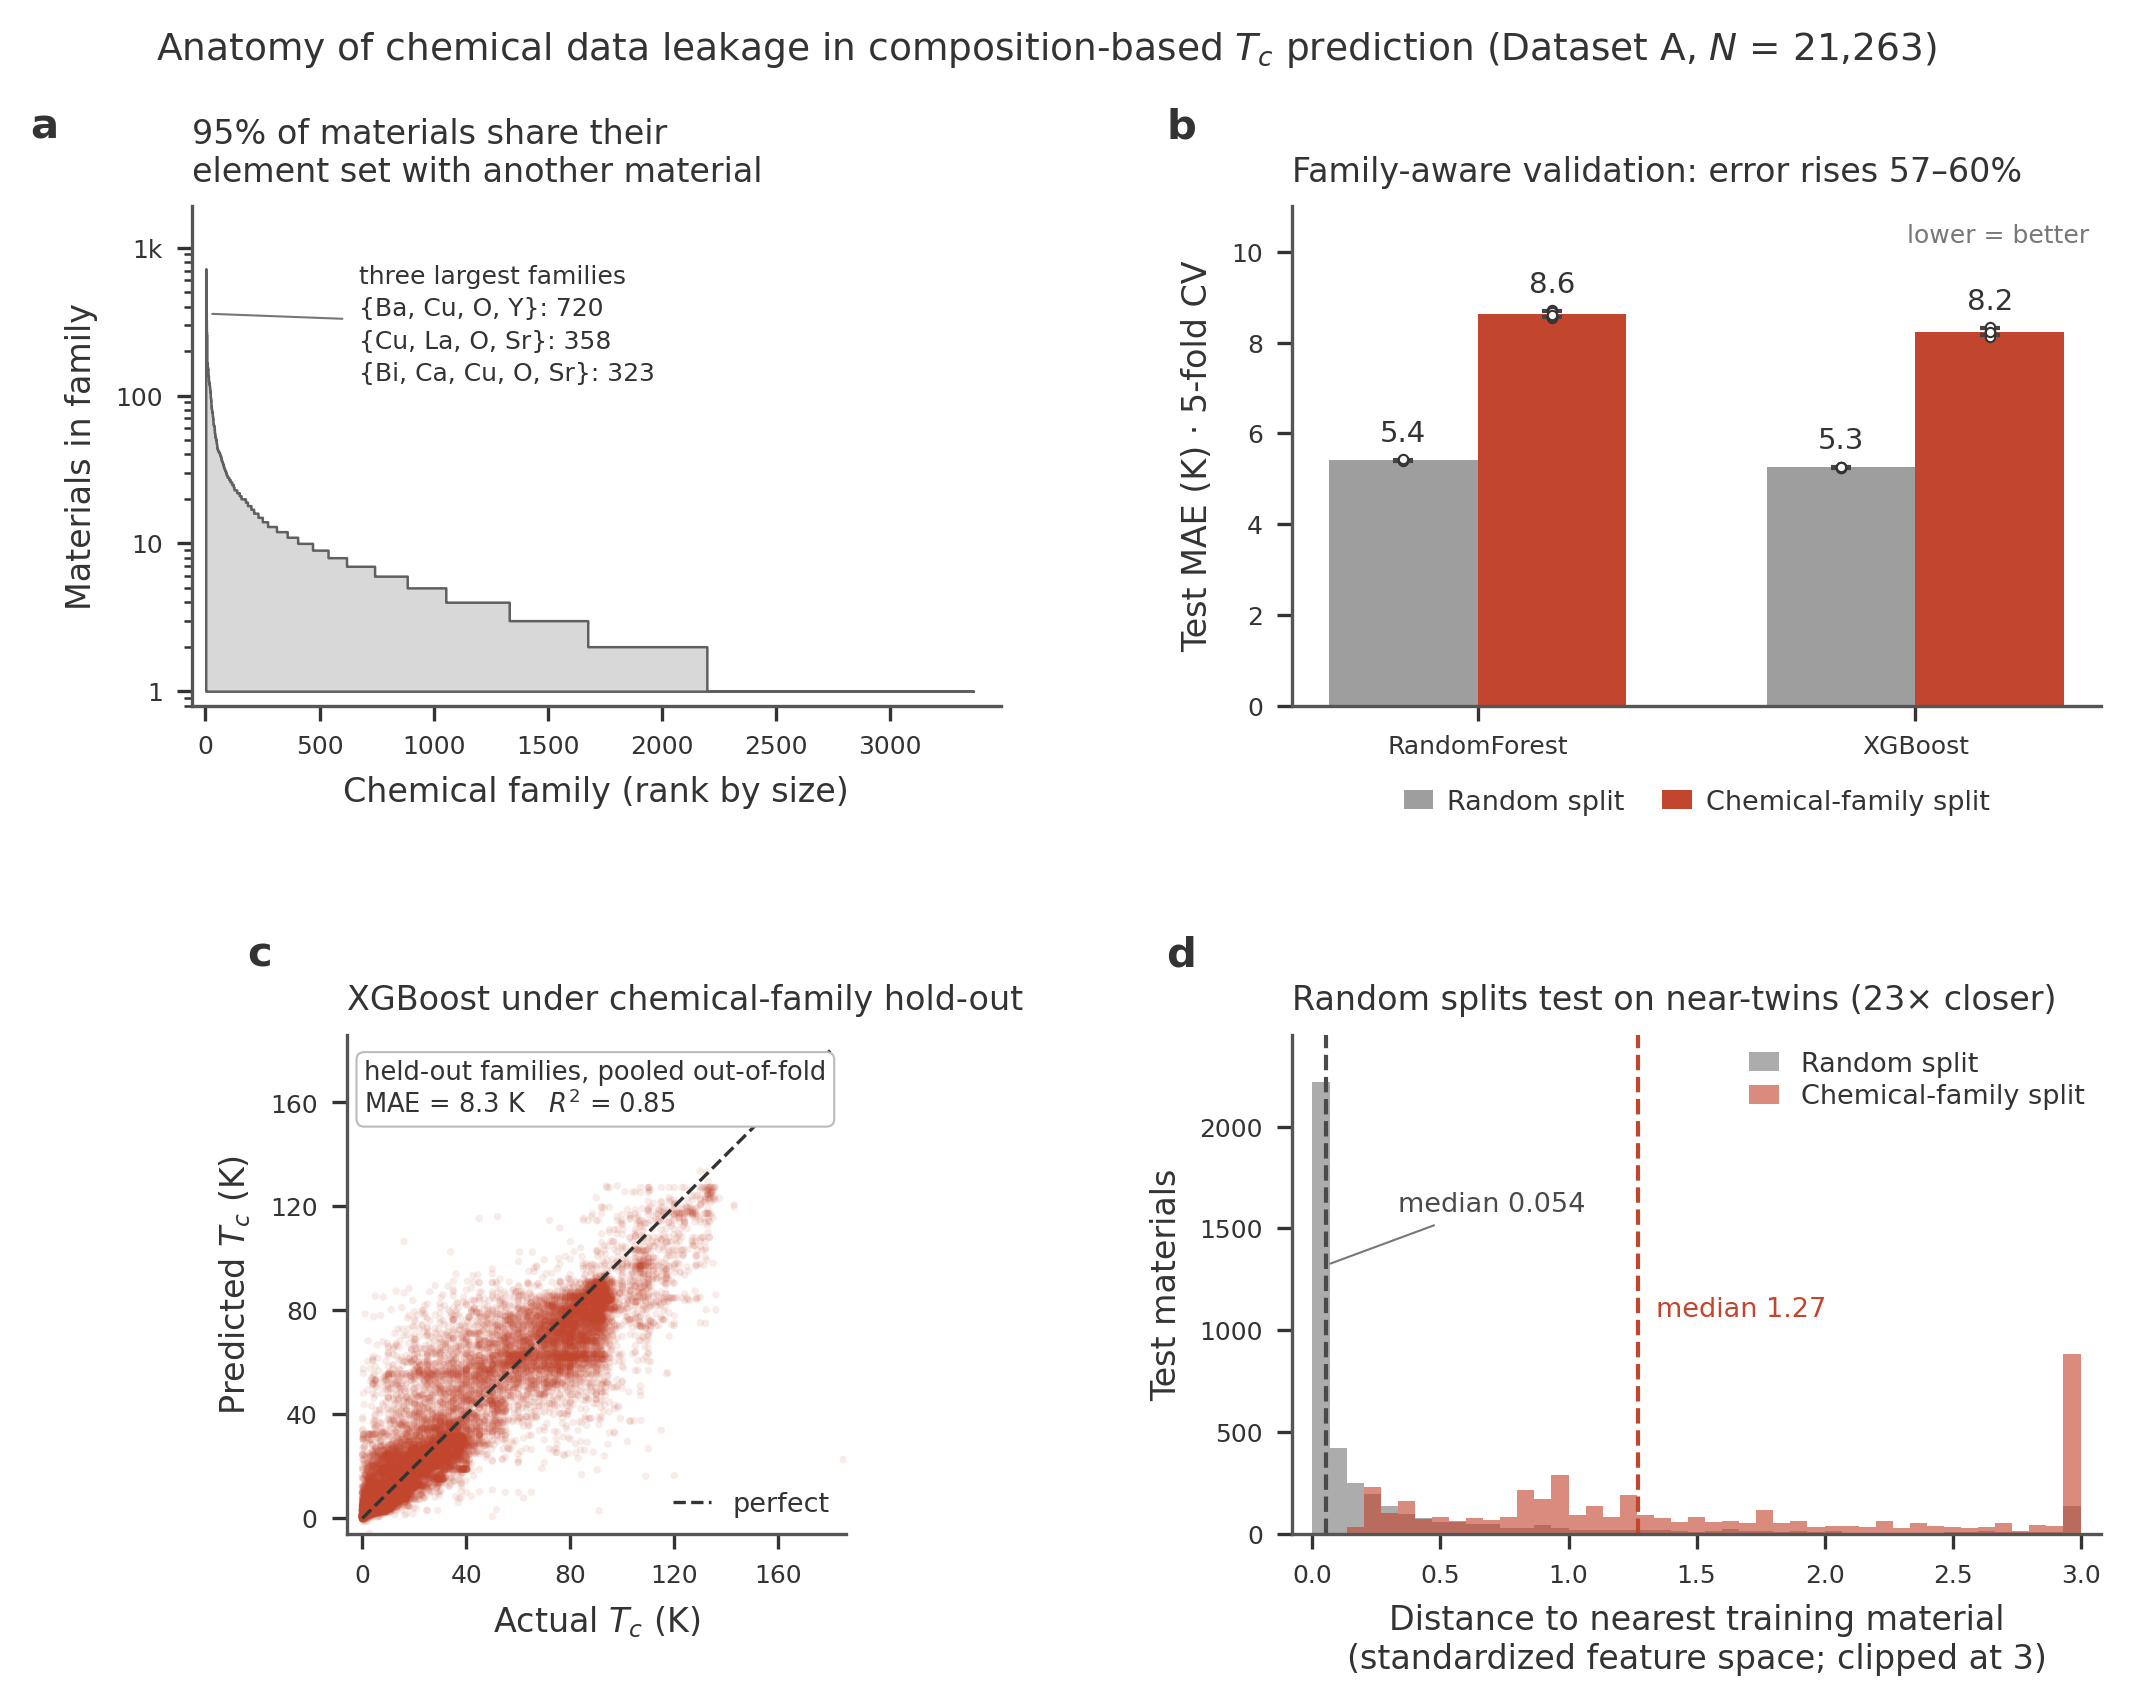
\includegraphics[width=0.98\textwidth]{figure1}
\caption{\textbf{Chemical leakage in Dataset~A is structural rather than incidental: most
materials share their exact element set with another material, so validation that ignores
families tests models on near-duplicates.} (a)~Distribution of chemical-family size, a family
being the set of materials with an identical constituent-element set ($n=\num{21263}$ materials
in $k=\num{3365}$ families; the largest, $\{$Ba, Cu, O, Y$\}$, holds \num{720} doping variants).
(b)~Test MAE under both protocols for both models; bars are means over five independent family
partitions, error bars the standard deviation across them, open circles the individual
partitions. (c)~Parity plot for XGBoost under chemical-family hold-out, pooling out-of-fold
predictions of the deterministic partition ($n=\num{21263}$ predictions, each from a model that
never saw the test material's family; MAE $=\SI{8.3}{\kelvin}$, $\Rsq=0.85$, both
cross-validated). (d)~Distance from each test material to its nearest training material in
standardised feature space for a single $80/20$ hold-out per scheme ($n=\num{4253}$ random and
\num{4344} family-split test materials; distances clipped at \num{3} for display). The median
test material is \num{23} times farther from its nearest training example under the family
split, which is the mechanism behind the error increase in~(b).}
\label{fig:anatomy}
\end{figure}

\subsection{Holding out chemical families inflates the error}
\label{sec:results-gap}

Table~\ref{tab:main} reports both protocols for both models and both datasets, together with the
family-mean null.

\begin{table}[t]
\caption{Pooled out-of-fold performance under random and chemical-family cross-validation.
The family-mean null uses no features: it predicts the training-fold mean $\Tc$ of the compound's
family. Under the grouped protocol every test family is unseen by construction, so the null
degenerates to a constant predictor and its $\Rsq$ is zero by definition---the informative
comparison is the random column, where the same lookup reaches $\Rsq = 0.80$ and $0.76$.}
\label{tab:main}
\centering
\setlength{\tabcolsep}{5pt}
\begin{tabular}{@{}llS[table-format=2.2]S[table-format=2.2]S[table-format=-1.3]@{}}
\toprule
Model & Split & {MAE (K)} & {RMSE (K)} & {$\Rsq$} \\
\midrule
\multicolumn{5}{@{}l}{\textit{Dataset A} (Hamidieh/UCI, $N=\num{21263}$, $k=\num{3365}$ families)}\\
Family-mean null & Random & 9.40 & 15.30 & 0.801 \\
Family-mean null & Chemical-family & 29.41 & 34.37 & -0.007 \\
XGBoost & Random & 5.23 & 9.17 & 0.928 \\
XGBoost & Chemical-family & 8.31 & 13.06 & 0.855 \\
Random forest & Random & 5.40 & 9.47 & 0.923 \\
Random forest & Chemical-family & 8.68 & 13.47 & 0.845 \\
\midrule
\multicolumn{5}{@{}l}{\textit{Dataset B} (Stanev/SuperCon, $N=\num{12440}$, $k=\num{3063}$ families)}\\
Family-mean null & Random & 8.19 & 13.94 & 0.764 \\
Family-mean null & Chemical-family & 22.67 & 28.74 & -0.003 \\
XGBoost & Random & 3.91 & 7.68 & 0.928 \\
XGBoost & Chemical-family & 6.17 & 10.99 & 0.853 \\
Random forest & Random & 4.33 & 8.31 & 0.916 \\
Random forest & Chemical-family & 6.52 & 11.56 & 0.838 \\
\bottomrule
\end{tabular}
\end{table}

The pattern is the same in both datasets. Enforcing family-disjoint folds raises XGBoost's MAE
from \SI{5.23}{\kelvin} to \SI{8.31}{\kelvin} on Dataset~A and from \SI{3.91}{\kelvin} to
\SI{6.17}{\kelvin} on Dataset~B, and lowers $\Rsq$ by \num{0.073} and \num{0.075}. The random
forest behaves identically. That two datasets with different curation, different size and
completely different featurizations agree to within a few hundredths of $\Rsq$ indicates that the
gap is a property of the prediction task, not of a particular data pipeline.

The nearest-neighbour diagnostic confirms the mechanism (figure~\ref{fig:anatomy}(d)). Under a
random hold-out the median distance from a test compound to its closest training compound is
\num{0.054} in Dataset~A; under a grouped hold-out of the same size it is \num{1.273}, a factor
of \num{23}. For Dataset~B the medians are \num{0.140} and \num{1.584}, a factor of \num{11}.
The random protocol is not evaluating extrapolation; it is evaluating recall of near-duplicates.

\subsection{The gap is stable across partitions}
\label{sec:results-robust}

A single partition could be unrepresentative, so we repeat both protocols over five independent
partitions (table~\ref{tab:robust}).

\begin{table}[t]
\caption{Robustness over five independent partitions. Both arms use shuffled splitters with
seeds \numrange{0}{4}, so the grouped partition itself varies between seeds and not only the
model initialisation. Inflation is computed per seed and then averaged. Uncertainties are
standard deviations across seeds.}
\label{tab:robust}
\centering
\setlength{\tabcolsep}{5pt}
\begin{tabular}{@{}llS[table-format=1.2]@{\,$\pm$\,}S[table-format=1.2]S[table-format=1.2]@{\,$\pm$\,}S[table-format=1.2]S[table-format=2.1]@{\,$\pm$\,}S[table-format=1.1]S[table-format=-1.3]@{\,$\pm$\,}S[table-format=1.3]@{}}
\toprule
& & \multicolumn{2}{c}{MAE random (K)} & \multicolumn{2}{c}{MAE grouped (K)}
& \multicolumn{2}{c}{Inflation (\%)} & \multicolumn{2}{c}{$\Delta\Rsq$} \\
\midrule
A & XGBoost & 5.25 & 0.01 & 8.24 & 0.07 & 56.9 & 1.6 & -0.071 & 0.003 \\
A & Random forest & 5.41 & 0.01 & 8.62 & 0.07 & 59.5 & 1.4 & -0.076 & 0.002 \\
B & XGBoost & 3.87 & 0.02 & 6.23 & 0.04 & 60.8 & 0.5 & -0.081 & 0.002 \\
B & Random forest & 4.32 & 0.01 & 6.58 & 0.02 & 52.5 & 0.6 & -0.081 & 0.002 \\
\bottomrule
\end{tabular}
\end{table}

MAE inflation ranges from \SI{52.5}{\percent} to \SI{60.8}{\percent} across the four
dataset--model combinations, and $\Delta\Rsq$ from \num{-0.071} to \num{-0.081}
(figure~\ref{fig:summary}(a),(b)). The
across-seed standard deviations are small---at most \num{1.6} percentage points of inflation---so
the effect is not an artefact of a fortunate partition. We note that these dispersions do
\emph{not} grow appreciably when the partition is allowed to vary rather than only the model
seed: pooled out-of-fold metrics average over the whole dataset, so redrawing the partition moves
them very little. The honest statement of run-to-run uncertainty for a single reported figure is
therefore the between-fold spread, which is considerably larger, and we quote it for the
per-fold screening metric in section~\ref{sec:results-screening}.

\begin{figure}[t]
\centering
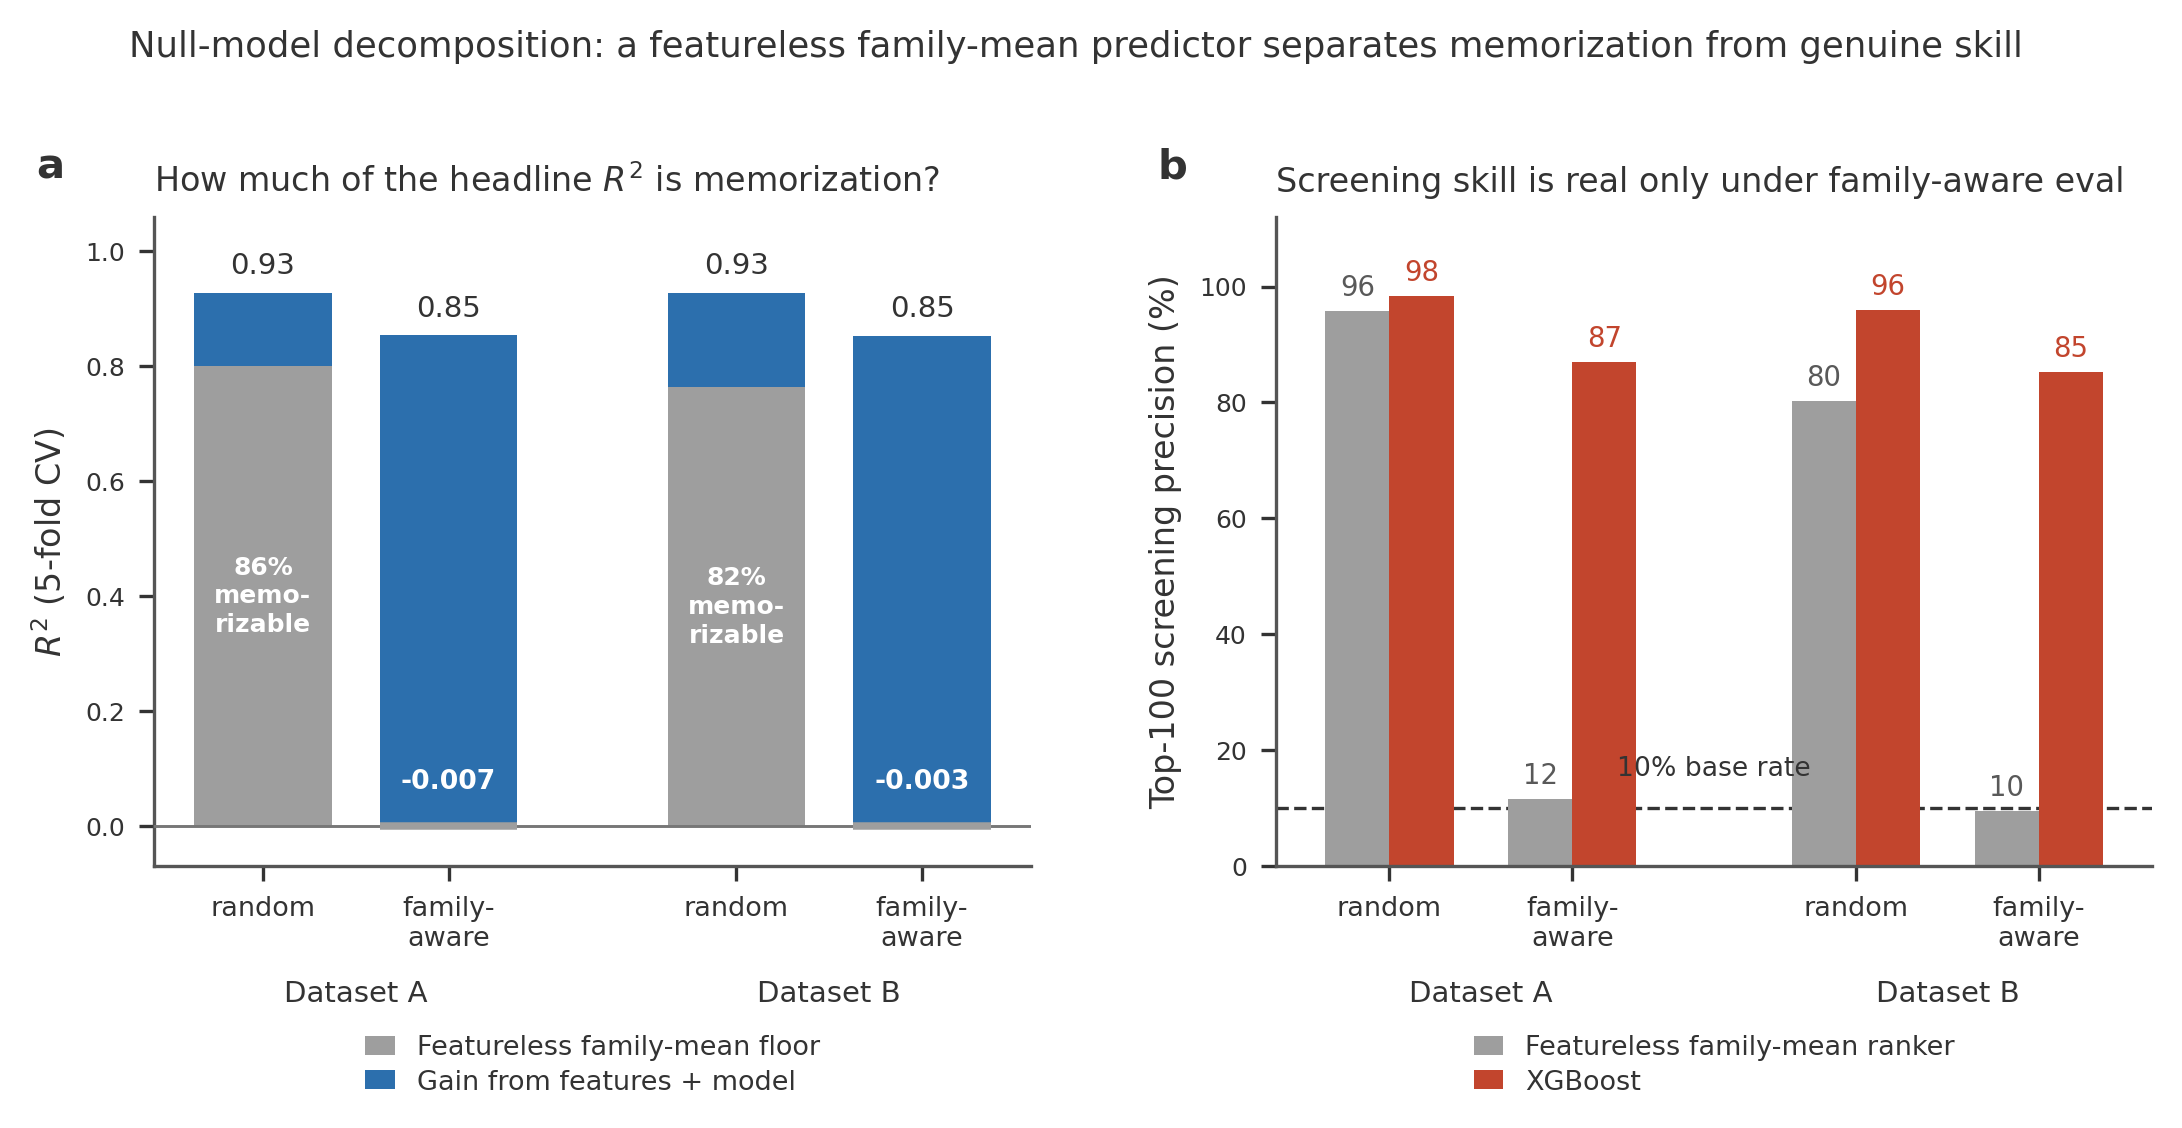
\includegraphics[width=0.98\textwidth]{figure2}
\caption{\textbf{A featureless predictor that returns only each family's mean $\Tc$ reproduces
most of the headline performance under random splitting, locating that performance in family
memorisation rather than in composition--property learning.} (a)~Decomposition of the
cross-validated $\Rsq$ into the part the family-mean null already achieves (grey) and the
increment contributed by features and model (blue), for both datasets under both protocols
(Dataset~A: $n=\num{21263}$, $k=\num{3365}$; Dataset~B: $n=\num{12440}$, $k=\num{3063}$). Under
random splitting the null alone reaches \SI{86}{\percent} (A) and \SI{82}{\percent} (B) of the
full model's $\Rsq$; under family-aware splitting it collapses to $\Rsq \approx 0$
($\num{-0.007}$ and $\num{-0.003}$, drawn as a baseline stub) because a held-out family has no
training mean to look up. All values are cross-validated; none is an oracle. (b)~Top-100
screening precision of the same featureless ranker against XGBoost. Under random splitting the
null ranks nearly as well as the model (\SI{95.8}{\percent} versus \SI{98.4}{\percent} on A);
under family-aware splitting it falls to \SI{11.6}{\percent} (A) and \SI{9.6}{\percent} (B), at
or near the \SI{10}{\percent} base rate, while XGBoost retains \SI{87.0}{\percent} and
\SI{85.2}{\percent}. The threshold is the 90th percentile of training-fold $\Tc$.}
\label{fig:null}
\end{figure}

\subsection{What the inflated number was measuring}
\label{sec:results-ceiling}

The gap tells us the conventional figure is optimistic. It does not by itself say what the
figure was measuring. Treating family identity as a clustering variable answers that
(table~\ref{tab:deff}).

\begin{table}[t]
\caption{Cluster structure of the two datasets. $\ICC$ is the intraclass correlation of $\Tc$
within a chemical family from a one-way random-effects ANOVA, equation~(\ref{eq:icc});
$\mathrm{deff}$ and $\Neff$ follow equation~(\ref{eq:deff}), reported for both the mean cluster
size $\bar m$ and Searle's $m_0$ for unequal clusters. $\eta^2$ is the in-sample fraction of $\Tc$
variance attributable to family identity, computed from family means over the full dataset; it is
not a cross-validated score and is not commensurable with the $\Rsq$ values in
table~\ref{tab:main}.}
\label{tab:deff}
\centering
\setlength{\tabcolsep}{6pt}
\begin{tabular}{@{}lS[table-format=5.0]S[table-format=4.0]S[table-format=1.3]S[table-format=1.3]S[table-format=1.2]S[table-format=1.2]S[table-format=4.0]S[table-format=4.0]S[table-format=1.2]@{}}
\toprule
& & & & & \multicolumn{2}{c}{deff} & \multicolumn{2}{c}{$\Neff$} & \\
\cmidrule(lr){6-7}\cmidrule(lr){8-9}
Dataset & {$N$} & {$k$} & {$\ICC$} & {$\eta^2$}
& {$\bar m$} & {$m_0$} & {$\bar m$} & {$m_0$} & {$\Neff/k$} \\
\midrule
A & 21263 & 3365 & 0.854 & 0.877 & 5.54 & 5.53 & 3836 & 3847 & 1.14 \\
B & 12440 & 3063 & 0.846 & 0.884 & 3.59 & 3.59 & 3466 & 3470 & 1.13 \\
\bottomrule
\end{tabular}
\end{table}

Two facts stand out. First, the intraclass correlation is \num{0.85} in both datasets: knowing
which doping series a compound belongs to determines most of its $\Tc$. Second, the resulting
effective sample size is essentially the number of chemical families. Dataset~A's \num{21263}
compounds carry the statistical information of \num{3847} independent observations against
\num{3365} families, a ratio of \num{1.14}; Dataset~B's \num{12440} carry \num{3470} against
\num{3063} families, a ratio of \num{1.13}. This is the expected limit: as $\ICC \to 1$,
$\mathrm{deff} \to m$ and hence $\Neff \to N/m = k$. At $\ICC = 0.85$ both datasets sit within
\SI{14}{\percent} of it. The choice of cluster size makes almost no difference---using
$\bar m$ instead of $m_0$ changes $\Neff$ by less than \SI{0.3}{\percent} in both
datasets---so the conclusion does not rest on the equal-cluster approximation.

The consequence for the headline metric is shown in figure~\ref{fig:ceiling}. In-sample, family
identity alone accounts for $\eta^2 = \num{0.877}$ of the variance in $\Tc$ on Dataset~A and
\num{0.884} on Dataset~B. This is not a score any model achieves or competes with---it is
computed with knowledge of every family's mean, and the cross-validated figures in
table~\ref{tab:main} are not commensurable with it. What it measures is the share of the target
that a categorical label already explains: on this task, seven-eighths of it.

The element-presence null makes a commensurable version of the same point, because it is
cross-validated on identical folds. With no statistical or Magpie descriptors whatsoever, binary
indicators of which elements are present reach $\Rsq = 0.847$ and \num{0.846} under a random
split, against \num{0.928} for the full featurization---about \SI{91}{\percent} of the headline
figure from element identity alone. The descriptor advantage does not widen when near-duplicates
are removed; in $\Rsq$ it narrows, from \num{0.081} to \num{0.052} on Dataset~A
(\num{0.803} versus \num{0.855} grouped) and from \num{0.082} to \num{0.074} on Dataset~B
(\num{0.779} versus \num{0.853}). Under both protocols and in both datasets, element identity
alone recovers more than nine-tenths of the regression score the full featurization achieves.
The screening metric behaves differently, and we return to it in
section~\ref{sec:results-screening}.

We stress the direction of this argument. It does not show that the models are learning nothing;
section~\ref{sec:results-screening} shows the opposite for the task that matters. It shows that
the conventional $\Rsq$ is a poor instrument for detecting what they learn, because most of the
variance it rewards is available from a categorical label.

\begin{figure}[t]
\centering
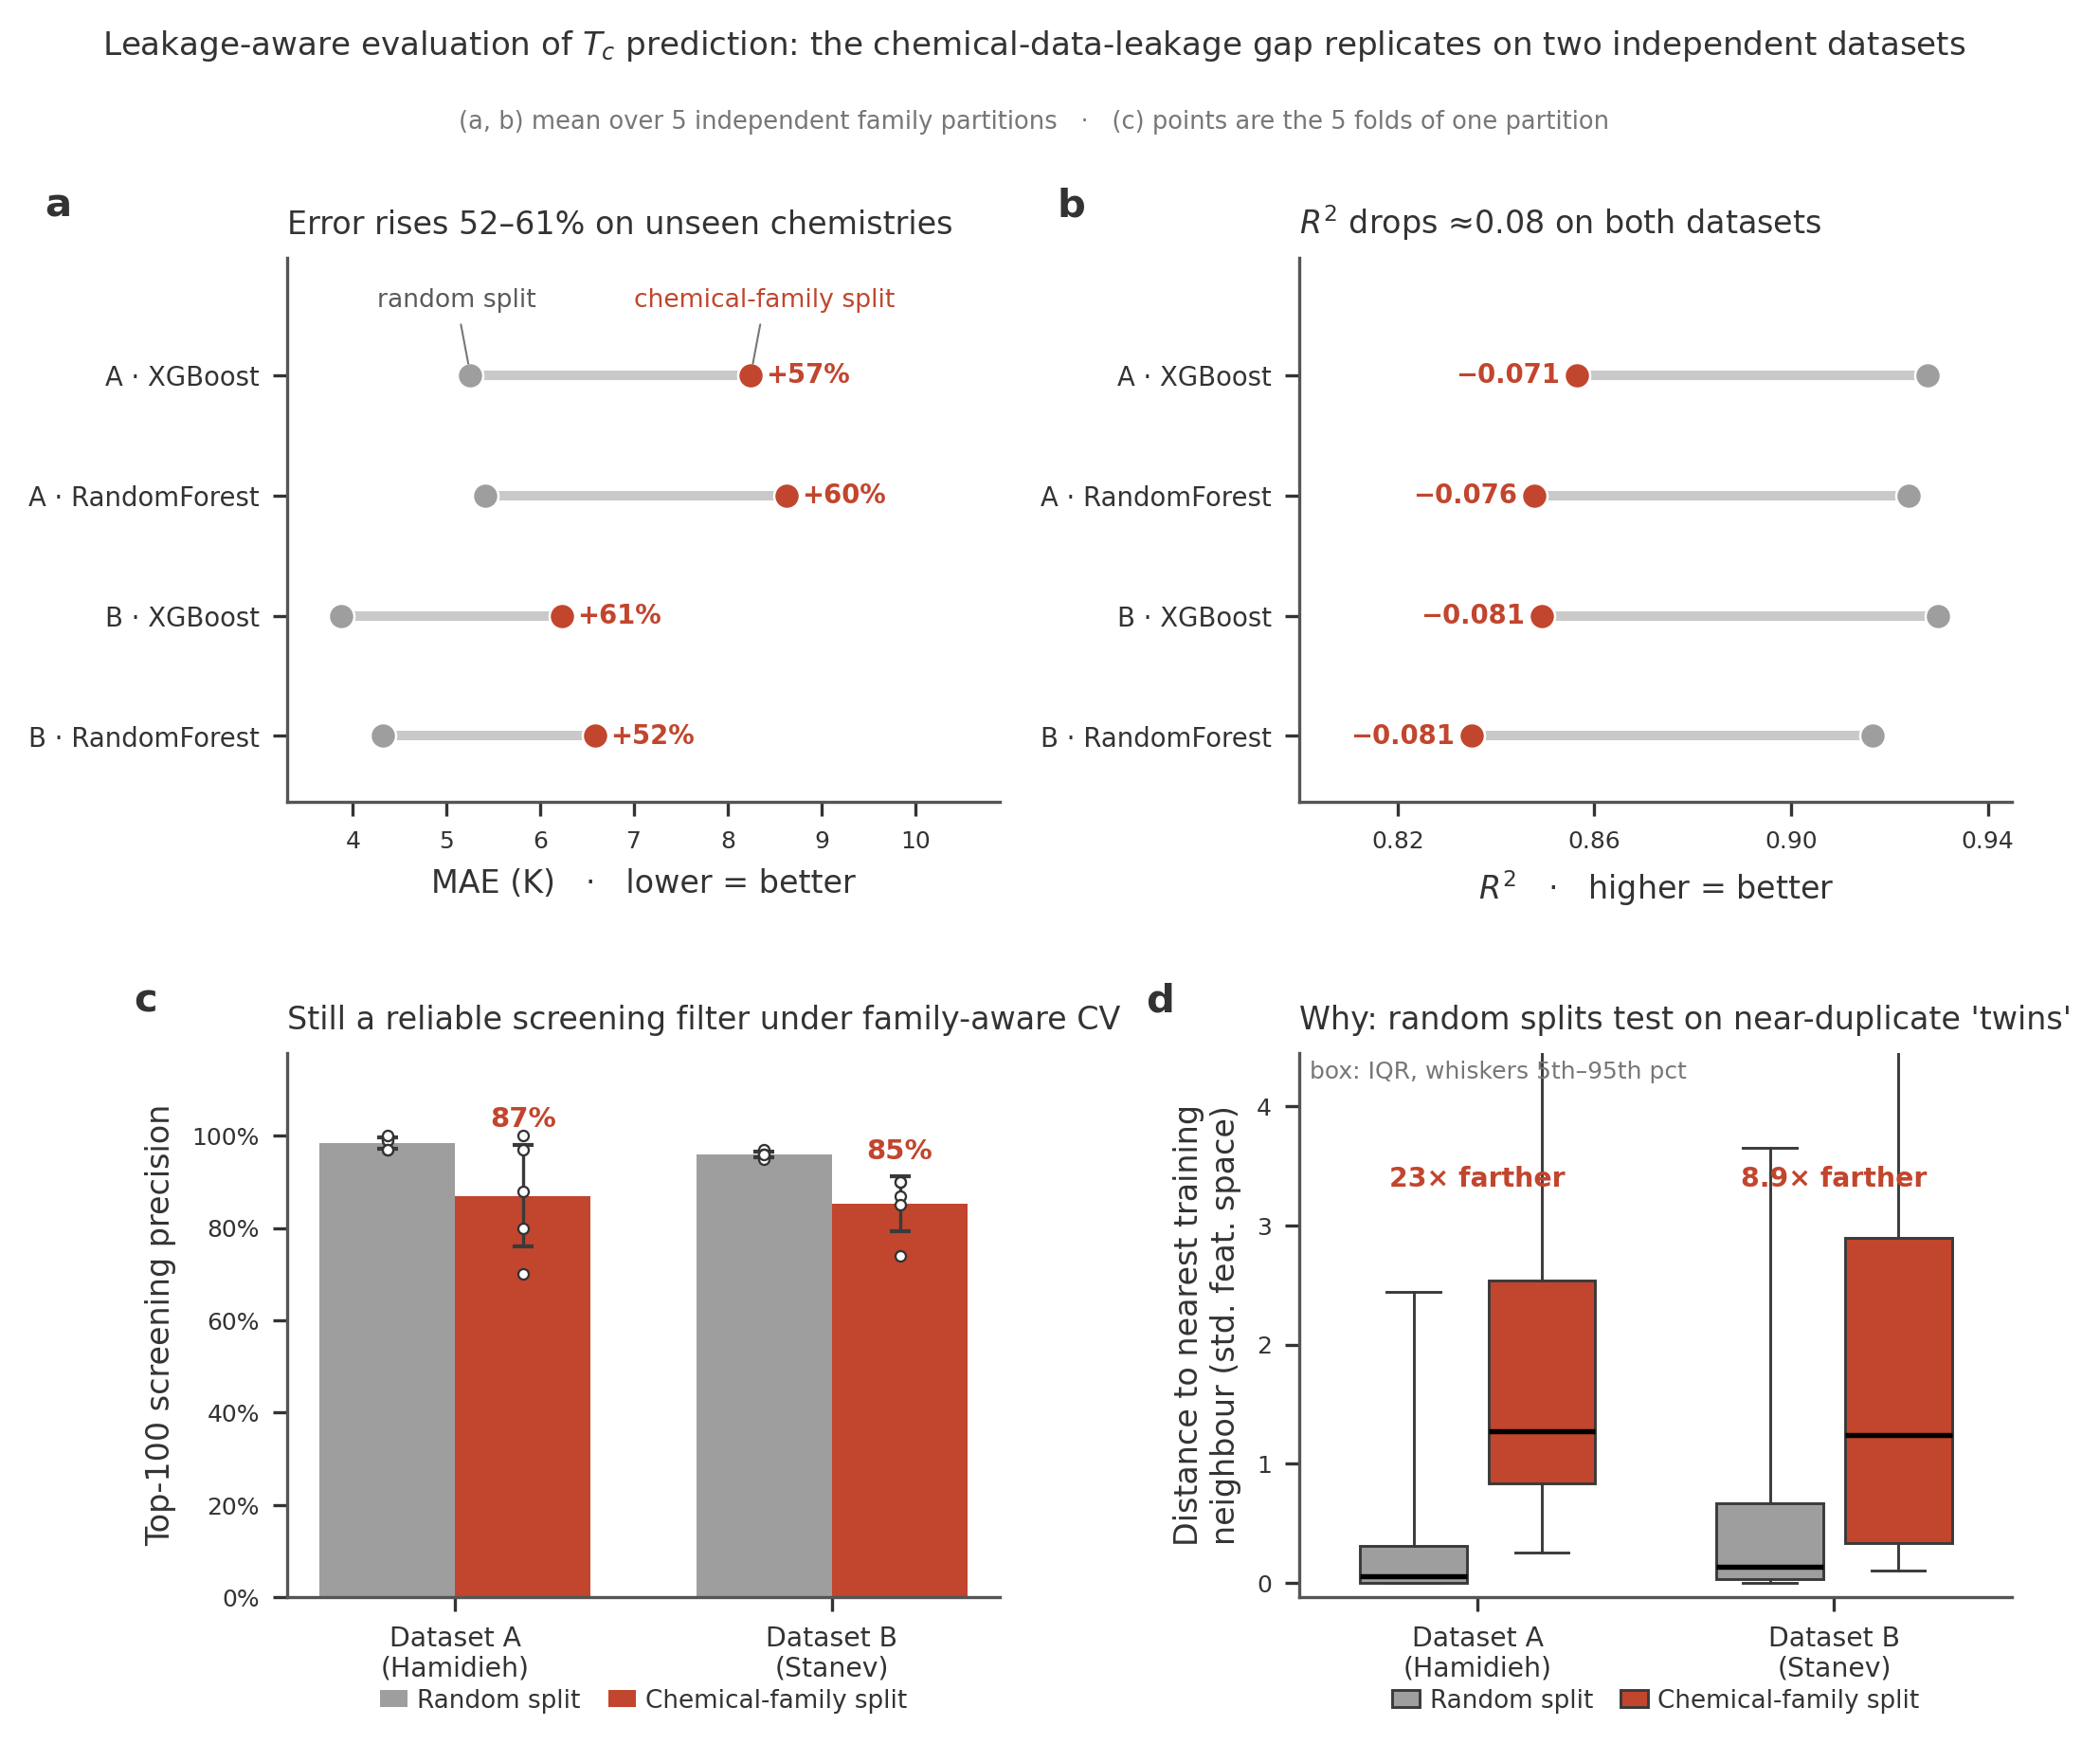
\includegraphics[width=0.98\textwidth]{figure3}
\caption{\textbf{The gap is not an artefact of one dataset, one featurization or one model: it
replicates across two independently constructed datasets, two model families and five
independent partitions.} (a)~Test MAE and (b)~$\Rsq$ for each dataset--model combination under
both protocols. Points are means over five independent partitions; the annotation gives the
paired per-seed MAE inflation and the signed change in $\Rsq$. MAE rises
\SIrange{52}{61}{\percent} and $\Rsq$ falls by \numrange{0.071}{0.081} in all four combinations.
(c)~Top-100 screening precision under both protocols; bars are the five-fold mean of the
deterministic partition, error bars its between-fold standard deviation, open circles the
individual folds. (d)~Distance to the nearest training neighbour in standardised feature space
for a single $80/20$ hold-out per scheme (A: $n=\num{4253}$ and \num{4344}; B: $n=\num{2488}$
and \num{2845} test materials); boxes show the interquartile range, whiskers the 5th--95th
percentile. All quantities except the distances in~(d) are cross-validated.}
\label{fig:summary}
\end{figure}

\begin{figure}[t]
\centering
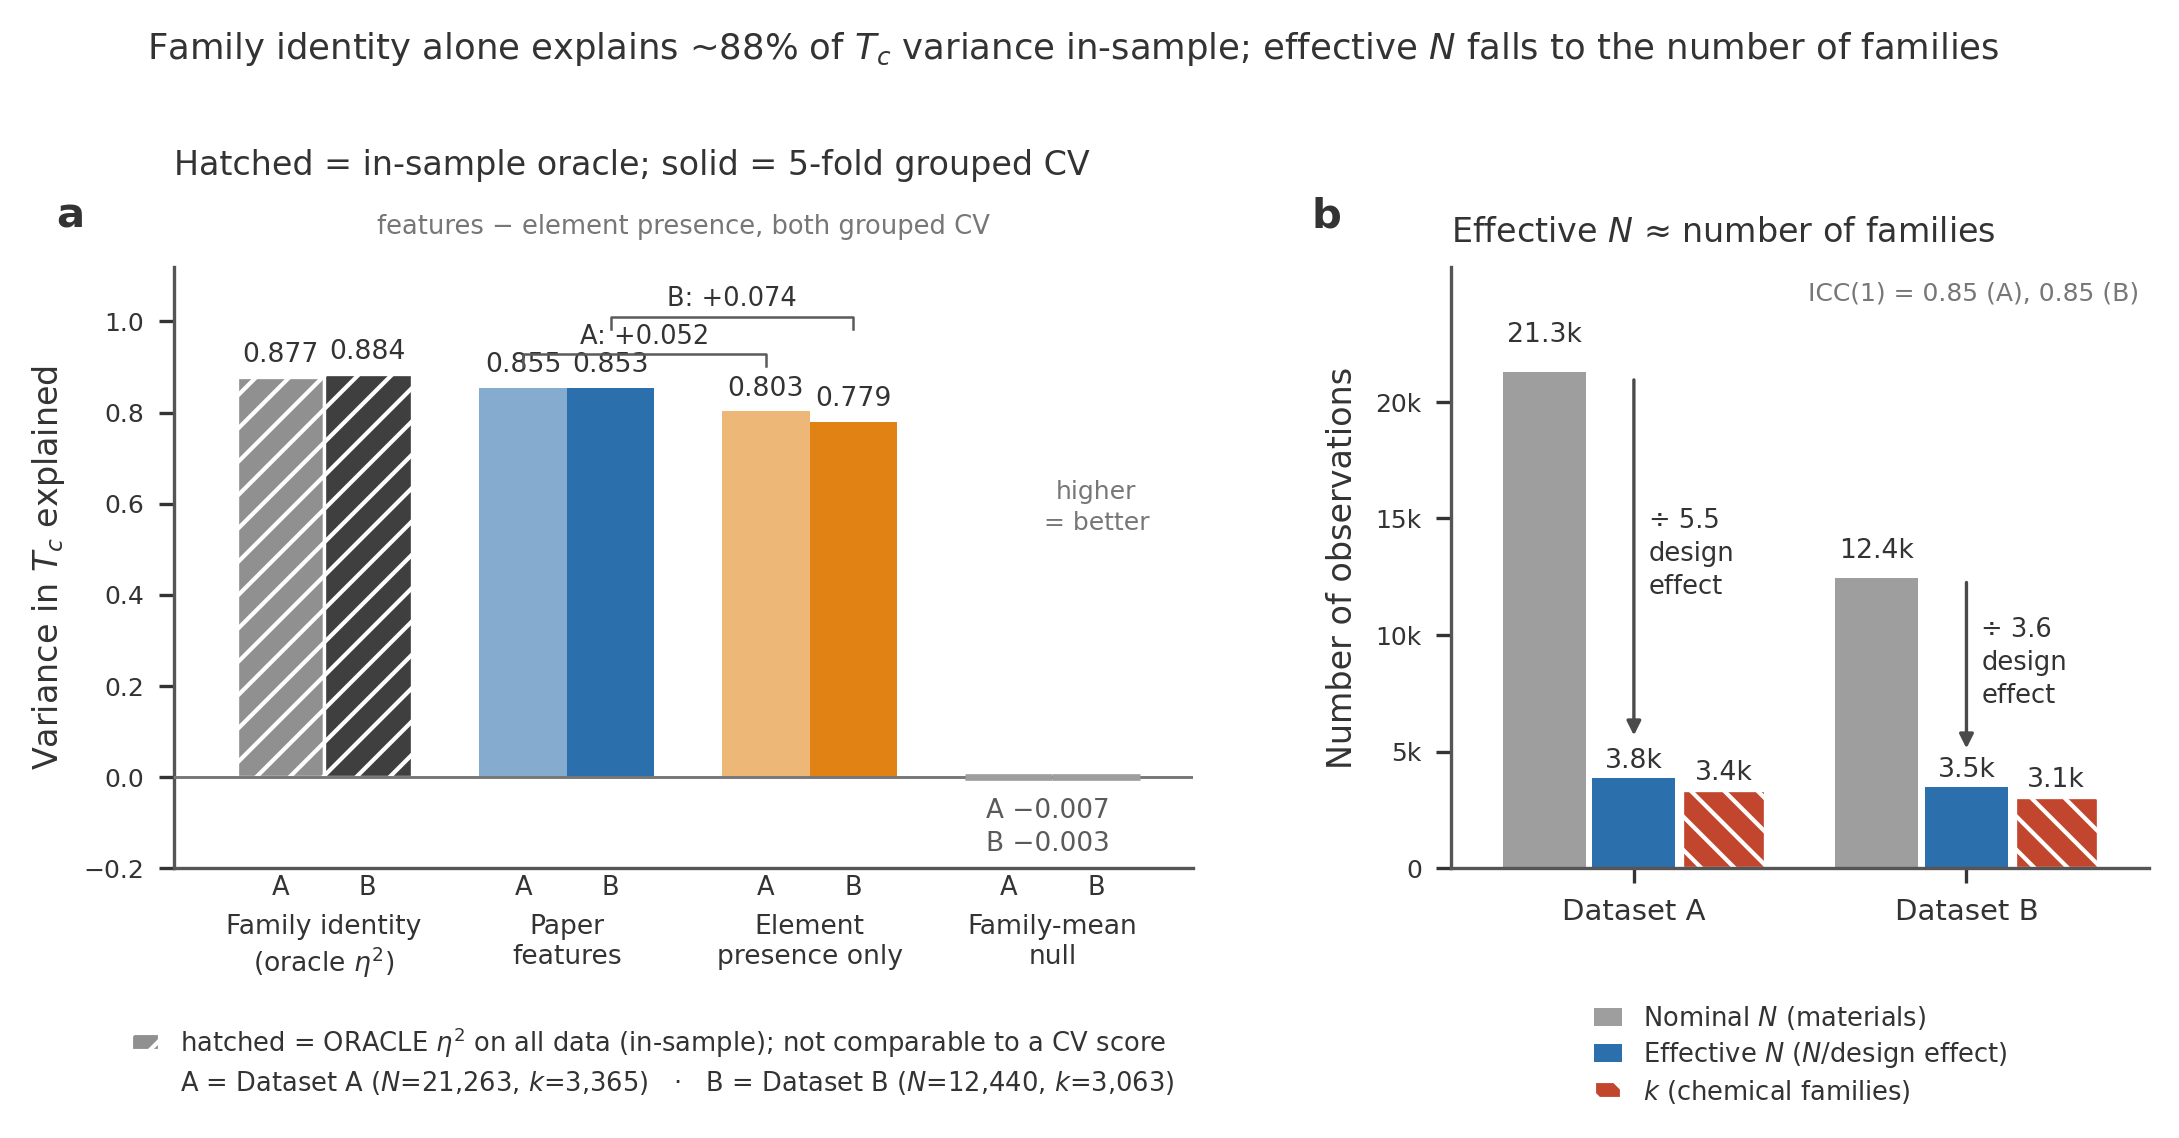
\includegraphics[width=0.98\textwidth]{figure4}
\caption{\textbf{Family identity alone accounts in-sample for about seven-eighths of the
variance in $\Tc$, and the clustering that produces this also reduces the effective sample size
to roughly the number of families.} (a)~Variance in $\Tc$ explained by four quantities, for
Dataset~A (light) and Dataset~B (dark). The leftmost pair is an \emph{oracle}: $\eta^2$ from a
one-way random-effects ANOVA using true per-family means computed on \emph{all} the data
(\num{0.877}, \num{0.884}). It is not a cross-validated score and not achievable by a model that
has not seen the test family; it is drawn hatched for that reason and must not be read as a
competitor to the bars beside it. The other three pairs are all cross-validated under grouped
five-fold CV: the paper's features (\num{0.855}, \num{0.853}), a null trained only on binary
element-presence indicators (\num{0.803}, \num{0.779}) and the family-mean null
($\num{-0.007}$, $\num{-0.003}$). The brackets mark the only commensurable difference in the
panel---features minus element presence, both grouped CV on identical folds---which is
\num{0.052} on Dataset~A and \num{0.074} on Dataset~B.
(b)~The same clustering expressed as a design effect. Effective $N$ is $N$ divided by
$1 + (m_0-1)\ICC$ with Searle's $m_0$; $k$ is the family count (hatched, being a count of design
units rather than observations). With $\ICC=\num{0.85}$ in both datasets the design effect is
\num{5.5} (A) and \num{3.6} (B), so \num{21263} materials carry about as much independent
information as \num{3847}, close to the \num{3365} families.}
\label{fig:ceiling}
\end{figure}

\subsection{Screening utility survives, and is genuinely descriptor-driven}
\label{sec:results-screening}

If most of the variance the regression metric rewards is already available from a family label,
does the practical application survive? Table~\ref{tab:screen} reports top-100 precision for the three-rung null ladder.

\begin{table}[t]
\caption{Top-100 precision under both protocols (per cent). The threshold is the 90th percentile
of training-fold $\Tc$, so the base rate is \SI{10}{\percent}. Values are means over five folds
with the between-fold standard deviation; the element-presence and full-model rows are additionally
verified over five independent partitions in the text.}
\label{tab:screen}
\centering
\setlength{\tabcolsep}{6pt}
\begin{tabular}{@{}llS[table-format=2.1]@{\,$\pm$\,}S[table-format=2.1]S[table-format=2.1]@{\,$\pm$\,}S[table-format=2.1]@{}}
\toprule
& & \multicolumn{2}{c}{Dataset A} & \multicolumn{2}{c}{Dataset B} \\
Predictor & Split & \multicolumn{2}{c}{} & \multicolumn{2}{c}{} \\
\midrule
Family-mean null & Random & 95.8 & 3.1 & 80.2 & 1.5 \\
Family-mean null & Chemical-family & 11.6 & 10.9 & 9.6 & 4.5 \\
Element presence & Random & 95.6 & 2.8 & 80.0 & 3.1 \\
Element presence & Chemical-family & 84.2 & 15.1 & 66.8 & 13.3 \\
Full model & Random & 98.4 & 1.2 & 96.0 & 0.6 \\
Full model & Chemical-family & 87.0 & 11.0 & 85.2 & 5.9 \\
\bottomrule
\end{tabular}
\end{table}

Under family-held-out validation the full model retains \SI{87.0}{\percent} precision on
Dataset~A and \SI{85.2}{\percent} on Dataset~B against a \SI{10}{\percent} base rate. Screening
utility is not destroyed by the corrected protocol: a campaign that synthesises the top-ranked
\num{100} candidates from an unseen chemistry would still find high-$\Tc$ materials in more than
four out of five attempts.

The null ladder shows that this skill is real rather than a lookup artefact
(figure~\ref{fig:null}). The family-mean null, which dominates under a random split
(\SI{95.8}{\percent} and \SI{80.2}{\percent}),
collapses to \SI{11.6}{\percent} and \SI{9.6}{\percent} under grouped validation---at or below
the base rate, since it cannot consult an unseen family. Element-presence indicators retain
substantial ranking power (\SI{84.2}{\percent} and \SI{66.8}{\percent}), so a large part of the
skill is attributable to chemical identity rather than to the descriptors' physics. But the
descriptors do contribute: measured over five independent partitions, discarding them costs
$7.7 \pm 1.0$ points on Dataset~A ($2.2\times$ the across-seed dispersion) and
$14.4 \pm 2.7$ points on Dataset~B ($9.9\times$), with the full model ahead in five seeds out
of five in both datasets.

The two datasets differ in how much the descriptors buy: the gap in Dataset~B is roughly twice
that in Dataset~A, a difference of \num{6.6} points at $3.3\times$ the across-seed dispersion
with disjoint ranges. We do not have a confirmed mechanism for the asymmetry. Dataset~A is the
more family-concentrated of the two (\SI{79.5}{\percent} versus \SI{66.7}{\percent} of compounds
in families of five or more), which would plausibly make element identity a stronger cue there,
but we have not tested that explanation and report the asymmetry as an observation.

\section{Discussion}

\subsection{What the numbers mean}

The single sentence that summarises this work is that \emph{the row is not the sample}. Superconductor
datasets are clustered samples of doping series, not simple random samples of compounds, and every
consequence measured here follows from that. The \SIrange{52}{61}{\percent} MAE inflation, the
$\ICC$ of \num{0.85}, the effective sample size that lands within \SI{14}{\percent} of the family
count, and the near-duplicate nearest-neighbour distances are four views of one fact.

The framing has a name outside materials informatics. Cluster sampling and its design effect are
standard in survey statistics, where reporting a nominal $N$ for a clustered sample is understood
to be an error rather than a modelling choice. Stating the problem this way has two advantages
over stating it as leakage: the diagnosis does not depend on which model is fitted or which
cross-validation protocol is used, and the remedy---analyse at the level of the cluster---is
already settled methodology.

\subsection{Relation to prior work}

That extrapolative validation is harder than interpolative validation for materials discovery is
established: Meredig \etal~\cite{meredig2018} demonstrated it with leave-one-cluster-out
cross-validation, and Kapoor and Narayanan~\cite{kapoor2023} place it within a broader pattern of
leakage-driven irreproducibility. The Matbench benchmarks~\cite{dunn2020,riebesell2024} similarly
separate regression accuracy from discovery utility. Our contribution is not the observation that
leakage exists but the specifics for this task: that the correct grouping variable for
superconductors is the constituent-element set, which is chemically interpretable and directly
verifiable rather than the output of an unsupervised clustering; that the resulting gap is
\SIrange{52}{61}{\percent} in MAE and replicates across two independently curated datasets and two
featurizations; that the inflation admits a model-independent expression as a design effect; and
that screening utility survives the correction.

\subsection{Scope and limitations}

Several boundaries should be stated plainly.

The family-mean null's collapse to $\Rsq \approx 0$ under grouped validation is a tautology, not
an empirical finding: with every test family unseen, the lookup returns the global training mean,
and a constant predictor has $\Rsq = 0$ by definition. We report it for completeness because it
calibrates the grouped column, but the informative half of that comparison is the random column,
where the same lookup reaches \num{0.80} and \num{0.76} without using any feature.

The oracle $\eta^2$ is computed with full knowledge of family means, including families a
cross-validated model never sees, so it is an in-sample descriptive quantity rather than a score
any protocol could return. It is not a competitor to the cross-validated figures and not a bound
on them---the random-split $\Rsq$ of \num{0.928} exceeds it, which is itself a symptom of the
leakage this paper measures. We mark it distinctly in figure~\ref{fig:ceiling} and never combine
it arithmetically with a cross-validated value.

The element-presence null removes stoichiometry and descriptor physics simultaneously, so it
cannot attribute the resulting drop to either alone. A third rung---presence plus fractions,
without Magpie descriptors---would separate them, and we have not run it.

We have measured only tree ensembles. Whether the gap widens with model capacity is a natural
question for graph and deep composition models, and we expect it to, but we have not measured it
and make no claim about it.

Finally, the corrected numbers are still retrospective. Family-held-out validation is a better
proxy for discovery than a random split, but the decisive test is prospective: predicting
compounds published after a cut-off date and measuring realised accuracy.

\subsection{Reproducibility}
\label{sec:repro}

The pipeline code, the deterministic family splits, the featurized Dataset~B checkpoint, the
result tables underlying every table and figure in this paper, and the scripts that render the
figures from those tables are released together for this revision (see Data availability).
Dataset~A is redistributed by UCI and is fetched by a script rather than bundled.

Three implementation details materially affect the numbers and are documented here because they
are not obvious from the protocol description. First, family labels must be assigned after row
filtering: \texttt{GroupKFold} breaks ties by label order, and with thousands of singleton
families a gapped labelling reassigns roughly \num{1800} of \num{2488} test rows per fold
relative to a contiguous one. Numbers produced from a gapped labelling are not fold-comparable
with numbers produced from a contiguous one even though the families are identical. Second, the
top-100 threshold must be stated explicitly, since the training-fold and whole-dataset
definitions differ by \num{0.4} points on Dataset~B. Third, top-100 precision is sensitive to the
XGBoost version: the algorithmic changes across major versions alter the ranking of predictions
even at fixed seed, and we therefore pin \texttt{xgboost==3.0.5} rather than a lower bound. The
figures reported here were produced with Python~3.13, numpy~2.3.3, scikit-learn~1.7.2,
xgboost~3.0.5 and matminer~0.9.2.

\section{Conclusion}

Composition-based $\Tc$ models are evaluated on datasets built from doping series, and splitting
those datasets at the level of the compound measures interpolation within a series rather than
generalisation to a new chemistry. Holding out whole chemical families inflates MAE by
\SIrange{52}{61}{\percent} and lowers $\Rsq$ by \numrange{0.071}{0.081}, consistently across two
independently curated datasets and two featurizations.

Expressed as a clustered sample, the same fact reads more sharply: with an intraclass correlation
of \num{0.85}, these datasets carry the statistical information of roughly their number of
chemical families---\num{3847} and \num{3470} effective observations for \num{21263} and
\num{12440} compounds---and family identity alone accounts in-sample for \SI{87.7}{\percent} and
\SI{88.4}{\percent} of the variance in $\Tc$. A cross-validated model trained only on which
elements are present, with no descriptors at all, reaches $\Rsq = \num{0.847}$ and \num{0.846}
under the conventional protocol, against \num{0.928} for the full featurization.

The practical conclusion is a recalibration rather than a dismissal. Screening precision under
family-held-out validation remains \SI{87.0}{\percent} and \SI{85.2}{\percent} against a
\SI{10}{\percent} base rate, and the descriptors demonstrably contribute to it. What changes is
the number that should be quoted: for Dataset~A, MAE $\approx \SI{8.3}{\kelvin}$ rather than
\SI{5.2}{\kelvin}. Obtaining it costs one additional cross-validation run, and we release the
splits so that it costs one command.

\section*{Data availability}

Code, deterministic chemical-family splits, the featurized Dataset~B checkpoint, all result
tables and the figure-generation scripts are available at
\url{https://github.com/Freakscode/superconductor-tc-leakage-eval} under the MIT licence, at the
tagged release accompanying this revision.
%% TODO antes de enviar: los scripts de figuras (results_v2/make_figures.py) y las tablas de
%% results_v2/ todavía NO están commiteados en ese repositorio. Hay que hacer push y crear el
%% tag v2.0 (+ DOI de Zenodo) para que esta frase sea cierta. Ver CAMBIOS_V2.md, sección
%% "Pendientes antes de enviar".
Dataset~A is the UCI Superconductivity Data Set~\cite{hamidieh2018}, retrieved by the included
\texttt{get\_datasetA.py}. Dataset~B derives from the curated list of Stanev
\etal~\cite{stanev2018}.

\begin{thebibliography}{99}

\bibitem{hamidieh2018}
Hamidieh K 2018 A data-driven statistical model for predicting the critical temperature of a
superconductor \textit{Comput. Mater. Sci.} \textbf{154} 346--54
\url{https://doi.org/10.1016/j.commatsci.2018.07.052}

\bibitem{stanev2018}
Stanev V, Oses C, Kusne A G, Rodriguez E, Paglione J, Curtarolo S and Takeuchi I 2018
Machine learning modeling of superconducting critical temperature
\textit{npj Comput. Mater.} \textbf{4} 29
\url{https://doi.org/10.1038/s41524-018-0085-8}

\bibitem{meredig2018}
Meredig B, Antono E, Church C, Hutchinson M, Ling J, Paradiso S, Blaiszik B, Foster I,
Gibbons B, Hattrick-Simpers J, Mehta A and Ward L 2018 Can machine learning identify the next
high-temperature superconductor? Examining extrapolation performance for materials discovery
\textit{Mol. Syst. Des. Eng.} \textbf{3} 819--25
\url{https://doi.org/10.1039/c8me00012c}

\bibitem{konno2021}
Konno T, Kurokawa H, Nabeshima F, Sakishita Y, Ogawa R, Hosako I and Maeda A 2021
Deep learning model for finding new superconductors \textit{Phys. Rev. B} \textbf{103} 014509
\url{https://doi.org/10.1103/PhysRevB.103.014509}

\bibitem{zeng2019}
Zeng S, Zhao Y, Li G, Wang R, Wang X and Ni J 2019 Atom table convolutional neural networks for
an accurate prediction of compounds properties \textit{npj Comput. Mater.} \textbf{5} 84
\url{https://doi.org/10.1038/s41524-019-0223-y}

\bibitem{court2020}
Court C J and Cole J M 2020 Magnetic and superconducting phase diagrams and transition
temperatures predicted using text mining and machine learning
\textit{npj Comput. Mater.} \textbf{6} 18
\url{https://doi.org/10.1038/s41524-020-0287-8}

\bibitem{xie2022}
Xie S R, Quan Y, Hire A C, Deng B, DeStefano J M, Salinas I, Shah R S, Fanfarillo L, Lim J,
Kim J, Stewart G R, Hamlin J J, Hirschfeld P J and Hennig R G 2022 Machine learning of
superconducting critical temperature from Eliashberg theory
\textit{npj Comput. Mater.} \textbf{8} 14
\url{https://doi.org/10.1038/s41524-021-00666-7}

\bibitem{sanna2024}
Sanna A, Cerqueira T F T, Fang Y-W, Errea I, Ludwig A and Marques M A L 2024
Prediction of ambient pressure conventional superconductivity above 80 K in hydride compounds
\textit{npj Comput. Mater.} \textbf{10} 44
\url{https://doi.org/10.1038/s41524-024-01214-9}

\bibitem{wrona2024}
Wrona I A, Jarosik M W, Szcz\k{e}\'sniak R and Durajski A P 2024 A recipe for an effective
selection of promising candidates for high-temperature superconductors among binary hydrides
\textit{Mater. Today Phys.} \textbf{46} 101499
\url{https://doi.org/10.1016/j.mtphys.2024.101499}

\bibitem{kapoor2023}
Kapoor S and Narayanan A 2023 Leakage and the reproducibility crisis in machine-learning-based
science \textit{Patterns} \textbf{4} 100804
\url{https://doi.org/10.1016/j.patter.2023.100804}

\bibitem{riebesell2024}
Riebesell J, Goodall R E A, Benner P, Chiang Y, Deng B, Lee A A, Jain A and Persson K A 2024
Matbench Discovery: A framework to evaluate machine learning crystal stability predictions
\textit{arXiv}:2308.14920
\url{https://doi.org/10.48550/arXiv.2308.14920}

\bibitem{dunn2020}
Dunn A, Wang Q, Ganose A, Dopp D and Jain A 2020 Benchmarking materials property prediction
methods: the Matbench test set and Automatminer reference algorithm
\textit{npj Comput. Mater.} \textbf{6} 138
\url{https://doi.org/10.1038/s41524-020-00406-3}

\bibitem{ward2018}
Ward L, Dunn A, Faghaninia A, Zimmermann N E R, Bajaj S, Wang Q, Montoya J, Chen J, Bystrom K,
Dylla M, Chard K, Asta M, Persson K A, Snyder G J, Foster I and Jain A 2018
Matminer: An open source toolkit for materials data mining
\textit{Comput. Mater. Sci.} \textbf{152} 60--9
\url{https://doi.org/10.1016/j.commatsci.2018.05.018}

\bibitem{ward2016}
Ward L, Agrawal A, Choudhary A and Wolverton C 2016 A general-purpose machine learning framework
for predicting properties of inorganic materials \textit{npj Comput. Mater.} \textbf{2} 16028
\url{https://doi.org/10.1038/npjcompumats.2016.28}

\bibitem{chen2016}
Chen T and Guestrin C 2016 XGBoost: A scalable tree boosting system
\textit{Proc. 22nd ACM SIGKDD Int. Conf. on Knowledge Discovery and Data Mining} 785--94
\url{https://doi.org/10.1145/2939672.2939785}

\end{thebibliography}

\end{document}
